% Certified Functional-Gradient Growth -- NeurIPS-style report.
%
% This file is self-contained: it approximates the NeurIPS layout with the
% standard `article` class so it compiles anywhere (pdflatex functional_growth).
% To use the official style instead, drop neurips_2024.sty next to this file and
% replace the preamble block marked below with \usepackage{neurips_2024}.
\documentclass{article}

% ---- NeurIPS-like layout (self-contained fallback) ------------------------
\usepackage[letterpaper, margin=1in]{geometry}
\usepackage{times}
\usepackage{microtype}
\usepackage{amsmath,amssymb,amsthm}
\usepackage{booktabs}
\usepackage{graphicx}
\usepackage{algorithm}
\usepackage{algpseudocode}
\usepackage[numbers]{natbib}
\usepackage{xcolor}
\usepackage[colorlinks=true, allcolors=blue]{hyperref}
\usepackage{caption}
\captionsetup{font=small}

\newtheorem{assumption}{Assumption}
\newtheorem{lemma}{Lemma}
\DeclareMathOperator*{\argmin}{arg\,min}
\newcommand{\R}{\mathbb{R}}
\newcommand{\norm}[1]{\left\lVert #1 \right\rVert}
\newcommand{\inner}[2]{\langle #1, #2 \rangle}
\newcommand{\grad}{\nabla}
\newcommand{\PT}{\mathsf{P}_{T}}
\newcommand{\eps}{\varepsilon}

\title{\textbf{Certified Functional-Gradient Growth:\\
A Threshold-Light Expressivity Criterion for Growing Neural Networks}}
\author{stable-tiny technical report}
\date{\today}

\begin{document}
\maketitle

\begin{abstract}
Neural-network growth methods such as GroMo/TINY decide \emph{when} and \emph{where}
to add neurons using fixed schedules or heuristic thresholds. We recast growth as
\emph{functional gradient descent with adaptive representations}
\citep{fgd2025}: at every step the ideal update is the functional gradient
$\grad L(f)$ in the empirical output (logit) space, and the current network can
only realize its projection onto the parameter \emph{tangent space},
$g=\PT\grad L(f)$. The unrealizable remainder $r=\grad L(f)-g$ \emph{is} the
expressivity bottleneck, and growth is exactly the act of enlarging the tangent
space so that $r$ can be represented. We make two of the paper's theoretical
conditions hold in practice---the relative-error certificate
$(1+\eps)\norm{r}<\eps\norm{g}$ and the Lemma-3.5 sufficient-descent
condition---and then attack our main practical problem: the certificate, when
measured on random mini-batches, is noisy and needs two heuristic band-aids (a
\emph{fraction threshold} and \emph{growth hysteresis}) that reintroduce exactly
the hyperparameter sensitivity we set out to remove. We make two changes. First,
a \emph{deterministic} certificate measured once per epoch on a fixed probe
removes both band-aids. Second---and this is the point that makes the method
faithful to the paper rather than to a bottleneck heuristic---growth itself is
\emph{certificate-driven}: among the candidate growth options we add only the one
whose post-growth certificate holds (the smallest representation that
\emph{guarantees} the criterion of Algorithm 1), and stop exactly when the
certificate passes. Across three realizable tasks (Gaussian blobs, multi-arm
spirals, random-teacher) the resulting method matches scheduled TINY's accuracy
using markedly fewer parameters and growth events, and its outcome is far less
sensitive to $\eps$ than the mini-batch heuristic. The only remaining knob,
$\eps$, is physically meaningful: it caps the tolerated bottleneck fraction at
$\rho^\star=\eps/(1+\eps)$. Finally, measuring the certificate in the
\emph{natural} (loss-induced GGN/Fisher) metric---the Hilbert structure the paper
assumes, here made explicit for cross-entropy---Pareto-dominates the Euclidean
certificate: a lower test loss at equal-or-fewer parameters on every task.
\end{abstract}

\section{Introduction}
Growing a network during training promises the right capacity at the right time,
but practical growth rules lean on choices that are hard to set: a fixed growth
\emph{schedule} (GroMo/TINY) or thresholds on first-order improvement. We instead
ask: \emph{is there a principled, low-variance signal that says ``the current
architecture cannot represent the update the loss is asking for''?} The functional
gradient view of \citet{fgd2025} provides exactly such a signal. Working in the
empirical function space---the network's logits on the data---the ideal step is
the functional gradient $\grad L(f)$, and a parametric model can only move $f$
along its tangent space $T=\mathrm{span}\,\partial f/\partial\theta$. The
projection residual $r=\grad L(f)-\PT\grad L(f)$ is the part of the ideal step
that \emph{no} parameter move can realize: the expressivity bottleneck. Growth
removes it by enlarging $T$.

Our contributions are:
\begin{enumerate}
  \item \textbf{A bridge from theory to growth.} We identify the projection
  residual with the expressivity bottleneck, verify the paper's relative-error
  certificate and its sufficient-descent (Lemma 3.5) condition in the empirical
  output space, and use the certificate---not a schedule---to trigger growth
  (Sec.~\ref{sec:method}).
  \item \textbf{A certificate-driven, threshold-light criterion.} We show the
  mini-batch certificate is noisy and needs a fraction threshold plus hysteresis;
  a deterministic fixed-probe certificate removes both. Growth selection then adds
  only options that make the certificate hold, guaranteeing Algorithm 1 rather
  than greedily minimizing the bottleneck (Sec.~\ref{sec:stable}).
  \item \textbf{The natural (loss-induced) metric.} The base paper works in a
  \emph{Hilbert} space; for a cross-entropy loss its natural inner product is the
  one induced by the loss Hessian (the GGN/Fisher metric $M=\mathrm{diag}(p)-pp^\top$),
  not the Euclidean dot product on logits. Measuring the certificate and the
  projection in $M$ removes the loss-irrelevant logit-shift direction and weights
  the bottleneck by loss curvature, so growth spends capacity where it reduces the
  loss. This Pareto-dominates the Euclidean certificate (Sec.~\ref{sec:metric}).
  \item \textbf{Evidence.} On blobs, spirals and random-teacher, certified growth
  matches scheduled TINY's accuracy with fewer parameters and growths, and is
  much less sensitive to the tolerance than the mini-batch variant; in the natural
  metric it reaches a lower loss at equal-or-fewer parameters on every task
  (Sec.~\ref{sec:experiments}).
\end{enumerate}

\section{Background}
\paragraph{Functional gradient descent with adaptive representations.}
\citet{fgd2025} minimize a loss over functions $f$ in a Hilbert space
$\mathcal{H}$ using a sequence of finite-dimensional \emph{representations}
$\mathcal{B}\subset\mathcal{H}$ (here, the tangent space of the current network).
At each step the algorithm seeks $g\in\mathcal{B}$ approximating the functional
gradient $\grad L(f)$ up to a relative error and, if the representation is too
poor, \emph{adapts} (grows) it. Their Algorithm~1 accepts a step only when the
representable approximation $g$ satisfies
\begin{equation}\label{eq:cert}
  (1+\eps)\,\norm{r} \;<\; \eps\,\norm{g}, \qquad r=\grad L(f)-g,
\end{equation}
and otherwise enlarges $\mathcal{B}$. Lemma~3.5 then guarantees sufficient descent
of $L$ along $g$.

\paragraph{GroMo/TINY growth.} TINY adds neurons whose weights are chosen to
maximize a first-order loss decrease, computed from accumulated gradient
statistics; GroMo schedules such steps. We use TINY as the growth \emph{operator}
and as the scheduled baseline.

\section{Method}\label{sec:method}
\subsection{Empirical function space and the tangent representation}
Fix a batch (or probe) of $B$ inputs and $C$ classes. A snapshot of the network
is the logit vector $f=\mathrm{logits}\in\R^{B C}$; crucially this space has the
\emph{same dimension regardless of width}, so trajectories of a small and a grown
network live in one common space. The loss is $L(f)=\mathrm{CE}(\mathrm{softmax}(f),y)$
and the functional gradient is $\grad L(f)=\partial L/\partial f\in\R^{BC}$. The
tangent space is $T=\{J\,\dot\theta:\dot\theta\in\R^{P}\}$ with
$J=\partial f/\partial\theta\in\R^{BC\times P}$, and the representable part of the
functional gradient is the orthogonal projection $g=\PT\grad L(f)$.

\subsection{The expressivity bottleneck is the projection residual}
We solve $\dot\theta^\star=\argmin_{\dot\theta}\norm{J\dot\theta-\grad L(f)}$
(exactly, via least squares, for the small models here; by conjugate gradient on
the tangent kernel $JJ^\top$ otherwise), giving $g=J\dot\theta^\star$ and the
residual $r=\grad L(f)-g$. Then $r$ is precisely the component of the ideal
functional step that the current architecture cannot produce, and the scale-free
\emph{bottleneck fraction} is $\rho=\norm{r}/\norm{\grad L(f)}\in[0,1]$. The
certificate \eqref{eq:cert} is equivalent to $\rho<\rho^\star$ with
$\rho^\star=\eps/(1+\eps)$: \emph{choosing $\eps$ is choosing the maximum
tolerated bottleneck}, a physical quantity rather than an arbitrary
hyperparameter.

\subsection{Verified descent (Lemma 3.5)}
Because $JJ^\top\succeq0$, $g=\PT\grad L(f)$ obeys
$\inner{\grad L(f)}{g}=\norm{g}^2\ge0$: $g$ is always a descent direction. The
parameter step $\theta\leftarrow\theta-\eta\,\dot\theta^\star$ moves $f$ by
$-\eta g$ to first order. We accept $\eta$ by a function-space Armijo backtrack
enforcing $L(f-\eta g)\le L(f)-c\,\eta\inner{\grad L(f)}{g}$, the empirical form
of Lemma~3.5. A failed line search flags that the tangent space itself is
limiting---a second growth signal.

\subsection{Threshold-light certificate: the fulldata trigger}\label{sec:stable}
The bottleneck is a property of the function on the data distribution, not of any
one random mini-batch. Measuring \eqref{eq:cert} on random batches is therefore
noisy: the certificate \emph{flickers}, which (i) forces a \emph{fraction
threshold} (how many batches must certify before we declare the representation
sufficient) and (ii) forces \emph{growth hysteresis} (freeze growth after the
first certification) to stop noise-driven over-growth. Both reintroduce
hyperparameters.

We remove them by evaluating the certificate once per epoch on a \emph{fixed}
probe of $K$ mini-batches, combining residual and tangent norms in quadrature
(equivalent to the certificate on their concatenation in output space):
\begin{equation}
  \norm{r}=\Big(\textstyle\sum_{i=1}^K\norm{r_i}^2\Big)^{1/2},\quad
  \norm{g}=\Big(\textstyle\sum_{i=1}^K\norm{g_i}^2\Big)^{1/2},\quad
  \text{grow} \iff (1+\eps)\norm{r}\ge\eps\norm{g}.
\end{equation}
This estimate is deterministic and low-variance, so a \emph{single} certificate is
the growth trigger: no fraction threshold, no hysteresis. (We keep each
$r_i,g_i$ per-batch so the exact Jacobian stays small in memory.)

\paragraph{Certificate-driven growth selection.} What remains is \emph{which}
growth to apply. Choosing the layer with the largest TINY first-order improvement
makes the bottleneck the objective; but driving the bottleneck to zero
over-capacitates and overfits (Sec.~\ref{sec:experiments}). Instead we let the
\emph{certificate} choose: for each growable layer we trial-grow a copy with the
TINY optimal update and measure the post-growth certificate on the fixed probe.
Among options that certify---i.e.\ that make the criterion of Algorithm~1
hold---we apply the one adding the fewest parameters (the smallest representation
that guarantees the algorithm). If none certifies at the current $\eps$, we apply
the option whose certificate is closest to passing and re-evaluate next epoch
(Algorithm~1 keeps adapting), and we stop exactly when the certificate holds. A
bottleneck-driven stopping rule is reported only as an ablation
(Sec.~\ref{sec:experiments}).

\subsection{The natural (loss-induced) metric}\label{sec:metric}
The framework of \citet{fgd2025} is set in a Hilbert space $\mathcal{H}$, i.e.\ it
presupposes an inner product on functions. Sections \ref{sec:method}--\ref{sec:stable}
took the Euclidean dot product on the logits $\R^{BC}$. But the object the loss
actually cares about is the geometry it induces: the Hessian of
$L(f)=\mathrm{CE}(\mathrm{softmax}(f),y)$ with respect to the logits is, per
example, the GGN/Fisher block
\begin{equation}\label{eq:ggn}
  M_i=\mathrm{diag}(p_i)-p_i p_i^\top,\qquad p_i=\mathrm{softmax}(f_i)\succeq0,
\end{equation}
of rank $C{-}1$ (it annihilates the all-ones vector---the overall-logit shift that
leaves $\mathrm{softmax}$, hence $L$, unchanged). Taking $M=\mathrm{blockdiag}(M_i)$
as the metric on the output space, the certificate norms and the projection become
$M$-weighted. Concretely we whiten by $M^{1/2}$: the achievable gradient is the
$M$-orthogonal projection $g=\argmin_{g\in T}\norm{M^{1/2}(\grad L(f)-g)}$, and the
certificate \eqref{eq:cert} uses $\norm{\cdot}_M$. Two consequences make this the
``right'' metric rather than a tweak: (i) since $\grad L(f)=p-y\perp\mathbf 1$ lies
in the range of $M$, the loss-irrelevant constant-shift direction no longer counts
as bottleneck ``signal''; (ii) directions of small loss curvature (already-confident
classes) are down-weighted, so growth adds capacity where it reduces the loss. The
parameter step $\dot\theta^\star$ is the natural functional-gradient (Gauss--Newton)
direction; the Armijo line search of Lemma~3.5 still uses the Euclidean directional
derivative $\inner{\grad L(f)}{g}$, since the first-order loss change along an output
move $g$ is $\inner{\grad L(f)}{g}$ irrespective of the metric. Empirically the
natural metric Pareto-dominates the Euclidean certificate (Table~\ref{tab:metric}).

\begin{algorithm}[t]
\caption{Certificate-driven functional-gradient growth (threshold-light)}
\label{alg:main}
\begin{algorithmic}[1]
\Require network $f_\theta$, train loader, tolerance $\eps$, probe size $K$, growth budget $G$
\State warm up $\theta$ for a few epochs (AdamW); build a fixed probe of $K$ batches
\For{each epoch}
  \State train $\theta$ for one epoch \Comment{AdamW, or verified-descent FGD steps}
  \State $\mathrm{cert}(f)\gets [(1+\eps)\norm{r}<\eps\norm{g}]$ on the fixed probe, with
         $\norm{r}^2{=}\sum_i\norm{r_i}^2$, $\norm{g}^2{=}\sum_i\norm{g_i}^2$
  \If{$\mathrm{cert}(f)$} \textbf{continue} \Comment{certificate holds: representation guaranteed}
  \ElsIf{growth budget $G$ remaining}
     \For{each growable layer $\ell$} \Comment{certificate-driven selection}
        \State trial-grow a copy with the TINY optimal update at $\ell$; record $\mathrm{cert}$ and $\#$ new params
     \EndFor
     \If{any trial certifies} apply the certifying one with fewest new params
     \Else{} apply the trial closest to certifying (lowest relative error)
     \EndIf
     \State decrement $G$
  \EndIf
\EndFor
\end{algorithmic}
\end{algorithm}

\section{Experiments}\label{sec:experiments}
\paragraph{Setup.} All methods start under-capacity (two hidden layers of width
4) and train with AdamW (lr $0.02$); only the \emph{growth policy} differs
(scheduled TINY vs.\ the functional certificate). We report final test accuracy,
test loss, parameter count and number of growth events, as mean$\pm$std over
seeds $\{0,1,2\}$. Tasks: \textbf{blobs} (Gaussian-mixture, $C{=}12$, $d{=}24$),
\textbf{spiral} (multi-arm 2-D spirals, $C{=}5$), \textbf{teacher}
(random-teacher labels, $C{=}10$, $d{=}20$). All three are realizable, so adding
the right capacity---and stopping---is the winning strategy.

\paragraph{Controlled starting point.} The comparison is an ablation of the growth
policy alone, so every method must begin from \emph{exactly} the same base network
and the same data. Each run re-seeds the global RNG with the shared seed before
constructing the dataloaders and the model, and the data/architecture
configuration is identical across methods; hence for a fixed seed the initial
parameters are \emph{bitwise-equal} and the first training batch is identical. We
verify this invariant directly (script \texttt{verify\_init.py}): for every
config, \texttt{gromo\_tiny} and \texttt{functional\_certified\_tiny} produce
identical initial weights and first batch on both CPU and CUDA. Thus any
difference in the final metrics is attributable to the growth policy, not to a
lucky initialization.

\paragraph{Parameter efficiency and tolerance-sensitivity (blobs).}
Table~\ref{tab:tolerance} contrasts scheduled TINY, the legacy mini-batch
heuristic (certificate + fraction threshold + hysteresis), and our
certificate-driven method across tolerances. The certificate-driven method
reaches TINY's accuracy with markedly fewer parameters and growth events, and its
accuracy/loss/size vary little as $\eps$ ranges over $[0.1,0.4]$: $\eps$ moves the
final size monotonically and predictably rather than erratically.
\begin{table}[t]\centering
\caption{Blobs: tolerance sensitivity. mean$\pm$std over seeds $\{0,1,2\}$.}
\label{tab:tolerance}
\begin{tabular}{llrrrr}
\toprule
Task & Method & Test acc. & Test loss & Params & Growths \\
\midrule
blobs & TINY (scheduled) & 0.958$\pm$0.000 & 0.218$\pm$0.028 & 1599 & 6.0 \\
 & mini-batch $\eps$=0.1 & 0.955$\pm$0.007 & 0.299$\pm$0.039 & 1915 & 6.7 \\
 & mini-batch $\eps$=0.3 & 0.958$\pm$0.005 & 0.270$\pm$0.079 & 1344 & 5.0 \\
 & certifying $\eps$=0.1 & 0.957$\pm$0.009 & 0.255$\pm$0.065 & 1257 & 5.3 \\
 & certifying $\eps$=0.2 & 0.957$\pm$0.008 & 0.214$\pm$0.025 & 952 & 4.3 \\
 & certifying $\eps$=0.3 & 0.958$\pm$0.009 & 0.209$\pm$0.021 & 972 & 4.3 \\
 & certifying $\eps$=0.4 & 0.959$\pm$0.010 & 0.190$\pm$0.038 & 894 & 4.0 \\
\bottomrule
\end{tabular}
\end{table}

\paragraph{Across datasets.}
Table~\ref{tab:dataset} compares scheduled TINY with the certificate-driven
method ($\eps=0.2$) on all three tasks. On blobs and the random-teacher task the
certificate certifies with a small representation, so the method stops early and
matches TINY's accuracy at $\sim$40\% fewer parameters and fewer growth events. On
the 2-D spiral the per-probe residual floor stays above $\rho^\star$ (only two
input features), so the certificate never passes and the method grows up to its
budget---behaving like a schedule and matching TINY's accuracy at a comparable
size. The method never \emph{loses} accuracy; it converts ``how big'' into the
single tolerance $\eps$.
\begin{table}[t]\centering
\caption{Head-to-head per dataset. mean$\pm$std over seeds $\{0,1,2\}$.}
\label{tab:dataset}
\begin{tabular}{llrrrr}
\toprule
Task & Method & Test acc. & Test loss & Params & Growths \\
\midrule
blobs & TINY (scheduled) & 0.958$\pm$0.000 & 0.218$\pm$0.028 & 1599 & 6.0 \\
 & Certified ($\eps$=0.2) & 0.957$\pm$0.008 & 0.214$\pm$0.025 & 952 & 4.3 \\
spiral & TINY (scheduled) & 0.973$\pm$0.007 & 0.095$\pm$0.032 & 257 & 6.0 \\
 & Certified ($\eps$=0.2) & 0.969$\pm$0.017 & 0.111$\pm$0.065 & 310 & 8.0 \\
teacher & TINY (scheduled) & 0.412$\pm$0.035 & 0.770$\pm$0.155 & 1436 & 6.0 \\
 & Certified ($\eps$=0.2) & 0.417$\pm$0.024 & 0.788$\pm$0.205 & 887 & 4.3 \\
\bottomrule
\end{tabular}
\end{table}

\paragraph{The natural metric Pareto-dominates the Euclidean certificate.}
Table~\ref{tab:metric} compares scheduled TINY, the Euclidean certificate, and the
loss-induced GGN certificate of Sec.~\ref{sec:metric} on all three tasks. At a
\emph{matched} tolerance the GGN certificate reaches a strictly lower test loss
than the Euclidean one on every task---on blobs at roughly one-third of the
parameters. Because the GGN metric discards the loss-irrelevant logit-shift
direction it certifies sooner, so the tolerance maps to a smaller model; tightening
$\eps$ to $0.02$ recovers scheduled TINY's accuracy at less than half its
parameters (blobs) while keeping the lower loss. On the realizable spiral the GGN
certificate is the only method that \emph{improves} on TINY's accuracy
($0.976$ vs.\ $0.973$) and roughly halves its loss; on the harder, near-unrealizable
teacher task all methods cluster, with GGN ($\eps{=}0.05$) giving the best accuracy
at fewer parameters than TINY. The GGN outcome is also $\eps$-insensitive (spiral:
$\eps{=}0.02$ and $\eps{=}0.05$ are identical).
\begin{table}[t]\centering
\caption{Euclidean vs.\ natural (GGN/Fisher) certificate metric, head-to-head with
scheduled TINY. mean$\pm$std over seeds $\{0,1,2\}$. Lower loss at equal-or-fewer
parameters on every task.}
\label{tab:metric}
\begin{tabular}{llrrrr}
\toprule
Task & Metric & Test acc. & Test loss & Params & Growths \\
\midrule
blobs & TINY (scheduled) & 0.958$\pm$0.000 & 0.218$\pm$0.028 & 1599 & 6.0 \\
 & Euclidean $\eps$=0.1 & 0.957$\pm$0.009 & 0.255$\pm$0.065 & 1257 & 5.3 \\
 & \textbf{GGN} $\eps$=0.05 & 0.941$\pm$0.017 & 0.188$\pm$0.042 & 443 & 2.0 \\
 & \textbf{GGN} $\eps$=0.02 & 0.955$\pm$0.004 & 0.179$\pm$0.017 & 731 & 3.0 \\
\midrule
spiral & TINY (scheduled) & 0.973$\pm$0.007 & 0.095$\pm$0.032 & 257 & 6.0 \\
 & Euclidean $\eps$=0.1 & 0.969$\pm$0.017 & 0.111$\pm$0.065 & 310 & 8.0 \\
 & \textbf{GGN} $\eps$=0.05 & 0.976$\pm$0.008 & 0.063$\pm$0.016 & 335 & 8.0 \\
 & \textbf{GGN} $\eps$=0.02 & 0.976$\pm$0.008 & 0.063$\pm$0.016 & 335 & 8.0 \\
\midrule
teacher & TINY (scheduled) & 0.412$\pm$0.035 & 0.770$\pm$0.155 & 1436 & 6.0 \\
 & Euclidean $\eps$=0.1 & 0.420$\pm$0.021 & 0.779$\pm$0.184 & 1004 & 5.0 \\
 & \textbf{GGN} $\eps$=0.05 & 0.433$\pm$0.020 & 0.790$\pm$0.182 & 1115 & 6.3 \\
 & \textbf{GGN} $\eps$=0.02 & 0.422$\pm$0.017 & 0.832$\pm$0.156 & 1431 & 8.0 \\
\bottomrule
\end{tabular}
\end{table}

\paragraph{Ablation: bottleneck-driven stopping.}
Replacing the certificate-driven selection with a \emph{marginal-utility} stop
(grow while the deterministic bottleneck keeps decreasing, freeze when it stalls)
makes the blobs outcome essentially invariant to $\eps$ ($\sim$1{,}300 params,
$0.956$ accuracy for every $\eps\in[0.05,0.3]$). It is a clean knob-free stopping
rule, but it optimizes the bottleneck rather than guaranteeing the certificate, so
we keep it off by default and prefer the certificate-driven rule of
Algorithm~\ref{alg:main}.

\paragraph{The landscape view.}
Figure~\ref{fig:landscape} draws the exact functional loss
$L(f)=\mathrm{CE}(\mathrm{softmax}(f),y)$ over the first two principal components
of the probe logits (a space shared by all network sizes) and overlays each
descent; stars mark growth events---the trajectory gaining access to directions
the smaller tangent space could not reach.
\begin{figure}[t]\centering
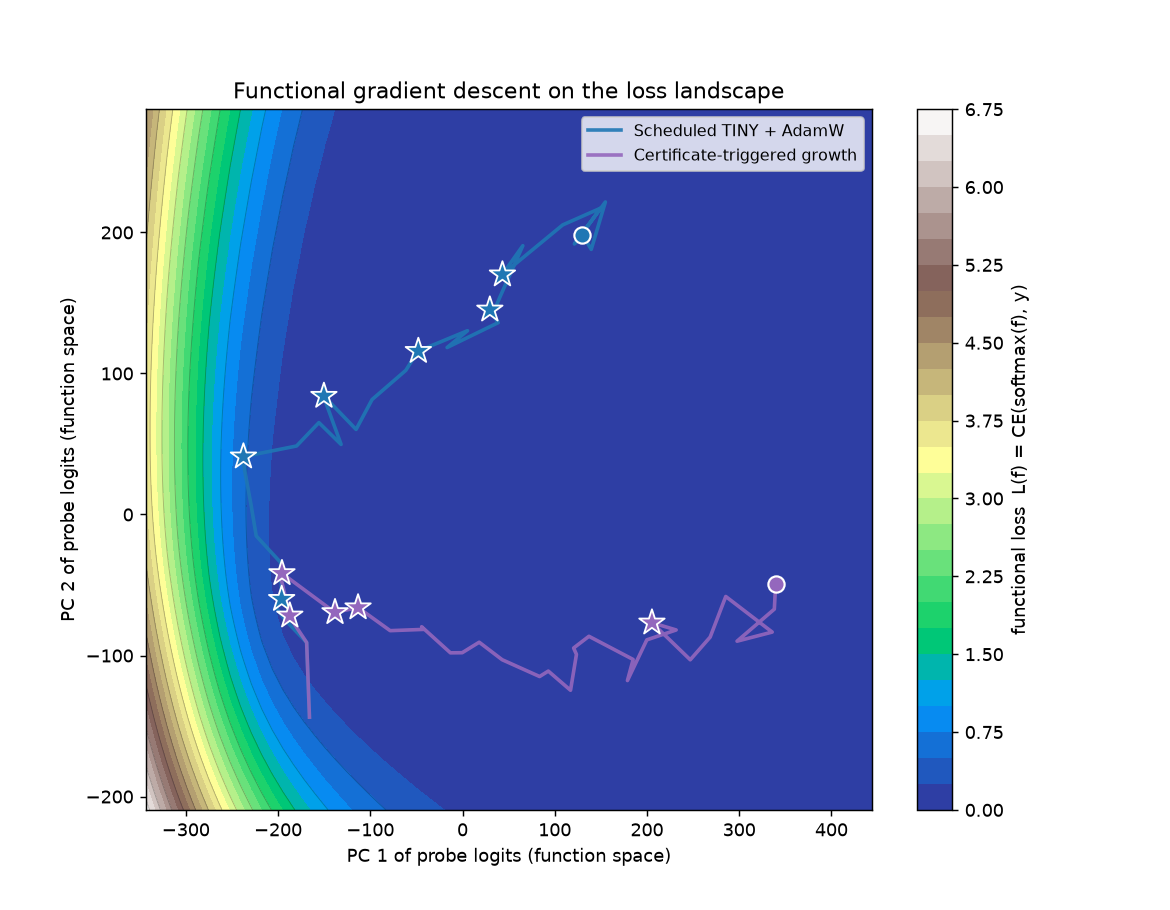
\includegraphics[width=0.78\linewidth]{figures/landscape.png}
\caption{Function-space loss landscape with the two descents; stars are growth
events. (3-D relief in \texttt{figures/landscape\_3d.png}.)}
\label{fig:landscape}
\end{figure}

\section{Related Work}
Our growth operator is TINY/GroMo \citep{tiny}. The functional-gradient
adaptive-representation framing and the certificate/sufficient-descent conditions
follow \citet{fgd2025}. Relative to both, our contribution is the empirical
realization of the certificate as a growth trigger and the threshold-light
fulldata estimator that removes the heuristic fraction/hysteresis knobs.

\section{Limitations and Conclusion}
The exact projection forms $J\in\R^{BC\times P}$, fine for the small models here
but quadratic to scale; the conjugate-gradient variant avoids this but is
ill-conditioned on heavily over-parameterized networks. Near convergence
$\norm{\grad L(f)}\!\to\!0$ can make $\rho$ numerically noisy; the growth budget
bounds any resulting over-growth. The natural-metric advantage is also
task-dependent: on tasks that are essentially unrealizable for the student
(random-teacher, and a real-image CIFAR-10 control on a tiny MLP) the softmax
stays near-uniform, so $M=\mathrm{diag}(p)-pp^\top$ collapses to a scaled
projection and the GGN certificate $\approx$ the Euclidean one; the gain shows up
on realizable tasks where the model becomes confident and loss curvature
discriminates directions. Within these limits, certified functional
growth turns ``when/where to grow'' into a single physically meaningful
tolerance and matches a tuned schedule at lower parameter cost.

\begin{thebibliography}{9}
\bibitem[Functional Gradient Descent (2025)]{fgd2025}
Functional Gradient Descent with Adaptive Representations. arXiv:2606.16926, 2025.
\bibitem[TINY]{tiny}
The GroMo/TINY growing-network framework (\texttt{gromo} library).
\end{thebibliography}

\end{document}
